\documentclass[10pt,a4paper]{article}
\usepackage[utf8]{inputenc}
\usepackage[italian]{babel}
\usepackage{amsmath}
\usepackage{amsfonts}
\usepackage{amssymb}
\usepackage{hyperref}
\usepackage{graphicx}
\usepackage{braket}
\usepackage[left=2cm,right=2cm,top=2cm,bottom=2cm]{geometry}
\newcommand{\rem}[1]{[\emph{#1}]}


\author{Belliardo Federico}
\title{``Dinamica dei Biliardini"- Rete delle idee}
\begin{document}

\maketitle


\begin{abstract}

Questa liste contiene alcune osservazioni, idee e dubbi raccolti durante la lettura di "Dinamica dei Biliardini" realizzato dalla Scuola Superiore di Udine.

\end{abstract}


\begin{itemize}

\item p.5 Avrei aggiunto delle immagini per chiarificare le definizioni date.

\item p.8 Avrei aggiunto delle immagini del cerchio per spiegare meglio la dimostrazione.

\item p.10 "siccome $a \neq b$, s è diverso da 0". Per una ellisse e una iperbole confocali $a = b$ non può mai succedere!

\item p.10 "È chiaro che questo lemma permette di ridurre la dimostrazione dell’enunciato seguente al solo caso dell'ellisse, dato che per ogni punto del piano passa un’ellisse confocale a un’iperbole data." Secondo me potevano essere un po' più specifici e fare un disegno: data una iperbole qualunque e un suo punto si può trovare una ellisse confocale passante per quel punto T. Basta infatti considerare $\phi^{-1} (|F_1 T - F_2 T|)$ e questa è l'ellisse desiderata. Data una qualunque retta passante per T si considera la perpendicolare. Se questa è tangente all'ellisse allora la sua ortogonale (la retta originaria) è tangente all'iperbole per il teorema sopra.

\item p.10 Separare nel lemma 2.4 la caratterizzazione della tangenza del lemma vero e proprio. Inoltre dopo aver concluso che per qualunque punto della retta $\phi (P) > \phi (A)$ si poteva fare un disegnino mostrando che i punti interni all'ellisse hanno $\phi (P) < \phi (A)$ (per quelli sull'ellisse vale l'uguale) e che quindi la retta interseca l'ellisse in un solo punto e per quanto detto alla fine della pagina prima essa è tangente (un solo punto di intersezione significa per forza tangenza).

\item p.11 Dimostrazione del lemma 2.4 non capisco perché l'ulteriore simbolo $\mathcal{E}$ per indicare l'ellisse. Non mi è chiarissimo come dimostra le due implicazioni diretta e inversa. Detto che la bisettrice è tangente basta dire che esiste un unica tangente, quindi data una certa retta che sappiamo essere tangente prendiamo la bisettrice (unica) dell'angolo esterno al vertice in quel punto e questa deve anche essere tangente, quindi deve coincidere con la precedente e quindi la retta originaria ha anche la proprietà di bisettrice. E' conveniente separare la caratterizzazione della tangente dal lemma perché diventa banale dire che una retta i cui due angoli acuti citati sono uguali ha la proprietà di bisettrice quindi di unica tangente.

\item p.11 Allineamento di $F_2, B, F_1'$ essere più specifici sul fatto che l'angolo compreso si somma a $\pi$.

\item Corollario 2.4.1 E' vero perché la normale biseca l'angolo tra i due fuochi, che è esattamente la condizione per la riflessione elastica da una superficie.

\item Corollario 2.4.2 Alla fine bisogna mettere insieme algebricamente tutte le relazioni tra gli angoli ricavate e ottenere la tesi.

\begin{figure}[!htb]
  \centering
  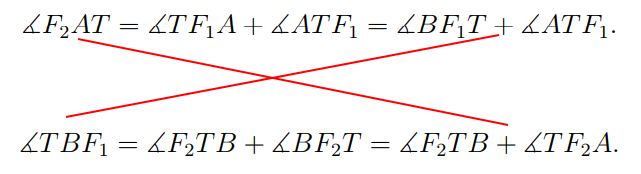
\includegraphics[scale=.5]{immagine1.png}
\caption{Sommare a chiasmo queste due relazioni.}
\label{trasporto}
\end{figure}

Si sommano e i sottraggo gli angoli come indicato sotto:

\begin{equation}
T B F_1 + B F_1 T + A T F_1 + F_1 T B - F_1 T B = F_2 T B + T F_2 A + F_2 A T + A T F_2 - A T F_2
\end{equation}

Si usa il fatto che la somma degli angoli interni di $F_1 B T$ e $ F_ 2 T A$ è uguale (ed è $\pi$) per ottenere:

\begin{equation}
ATF_1 - F_1TB = F_2TB-ATF_2
\end{equation}

dalla quale:

\begin{equation}
ATF_1 + ATF_2 = F_2TB + F_1TB
\end{equation}

ma i due angoli sommati per ogni membro di destra e di sinistra differiscono per la stessa costante dunque: $ATF_1 = F_2TB$.

\item p.12 Proposizione 2.5: per essere consistenti con le definizioni precedenti su come si prende l'angolo $\alpha$ bisogna specificare che senza perdita di generalità la traiettoria è diretta verso $F_2$.
 
\item p.13 Teorema 2.6-Dimostrazione. Si afferma che per il lemma 2.4 $A_0A_1F_1 = F_2A_1A_2$. Questo segue più che altro dalla caratterizzazione alternativa della tangente, per cui la normale biseca $F_1 A_1 A_2$. Ma per la definizione di riflessione elastica i due segmenti di traiettoria formano lo stesso angolo rispetto alla normale, ne segue $A_0A_1F_1 = F_2A_1A_2$.

\item p.13 Teorema 2.6-Dimostrazione. Il fatto che l'ellisse tangente al segmento $A_0 A_1$ sia anche tangente al successivo mostra che anche $A_1 A_2$ non interseca $F_1 F_2$ quindi la costruzione per induzione si può estendere a tutti i segmenti dell'orbita. Similmente una retta tangente ad una iperbole in qualsiasi punto interseca sempre $F_1 F_2$.

\item p.14 Teorema 2.8. Non è necessaria la convessità stretta: la traiettoria scelta può anche avere parti con supporto nel bordo del biliardino.

\item p.16 Dimostrazione lemma 2.9. Si dice che un'eventuale altra intersezione di $\tau$ con $\mathcal{C}$ sarebbe contenuta in $\mathcal{C_0}$. Dato questo punto $K$ se esso fosse fuori da $\mathcal{C_0}$ esso si troverebbe nella parte opposta di semipiano identificato dalla retta AB rispetto a $P$. Per attraversare il semipiano la retta $KP$ dovrebbe rimanere completamente nel biliardo. Pertanto sulla retta di separazione tra i due semipiani essa deve intersecare internamente il segmento $AB$. La tangente ad una ellisse in ogni punto non può intersecare il segmento che congiunge i fuochi.

\item p.16 "La chiusura di S contiene anche n-ple associate a poligoni con meno di n
lati": nel senso che gli stessi segmenti possono essere percorsi più volte, cioè possono sovrapporsi.

\item p.16 E' implicito che una retta che intersechi una figura convessa in un solo punto ne sia la tangente in quel punto.

\item p.16 "per i lemmi 2.4 e 2.9, in qualsiasi traiettoria di biliardo che li
contiene, il segmento AB ha come successivo il segmento BC": per quanto detto prima vi è una ellisse con fuochi A e C passante per B tale che le tangenti a $\mathcal{C}$ e all'ellisse coincidono. Dunque la normale in quel punto all'ellisse (e al biliardino convesso) biseca l'angolo $ABC$ ma questa è esattamente la condizione necessaria per il rimbalzo elastico. Segue che la il poligono di $n$ lati trovato è una possibile orbita di biliardino.

\item p.18 "Quindi, se un insieme $X \subseteq [0, 1[^{2}$ è denso per la metrica euclidea, allora è denso anche per
la metrica del toro". Palle di raggio sufficientemente piccolo per la metrica euclidea e per quella del toro sono indistinguibili. Dunque un insieme $X$ denso per la metrica euclidea è tale per cui per ogni punto data una palla arbitrariamente piccola centrata in esso un punto di $X$ è contenuto all'interno. Ma la palla data è anche palla dello stesso raggio per la metrica del toro e viceversa.

\item p.19 Proposizione 3.1. Dato un punto di $[0, 1[^{2}$ è sufficiente considerare la retta orizzontale passante per esso cioè $\mathcal{L}_{h}$: questa conterrà punti della traiettoria arbitrariamente vicini al punto iniziale dato.

\item p.19 "Siccome i differenziali di tali riflessioni affini sono riflessioni vettoriali rispetto a due rette
ortogonali, allora esse generano un gruppo di isometrie di ordine 4. Segue che, prese quattro copie
del quadrato con un vertice in comune, tutte le altre copie sono ottenute con una traslazione di
una di queste quattro.". Questa frase non l'ho capita. Ma il succo dovrebbe essere che considerando quattro quadrati adiacenti della data tassellazione tutto il piano si può ottenere per traslazione. Inoltre possiamo identificare i quattro quadrati con il toro e dunque le traiettorie del biliardo con i flussi positivi sul toro.

\item p.20 Biliardi poligonali. Si afferma che: "Segue che G(P) è isomorfo al gruppo diedrale di ordine 2N , da cui si capisce che le
possibili direzioni sono al massimo 2N": non mi è chiaro il significato di questa frase, proverò a leggere la referenza originale.

\item p.23 Biliardo non illuminabile di Penrose: un raggio di luce che parte dalla zona C è costretto ad attraversale la linea dei fuochi e pertanto comunque sia la sua evoluzione (anche se colpisce i due "funghi") esso è costretto a rimanere all'interno di un iperbole (che può cambiare di rimbalzo in rimbalzo!) ma in ogni caso non può raggiungere le zone primate. Se parte da A o B può rimanere intrappolato in una ellisse o in una iperbole ma non può finire nelle regioni primate dalla parte opposta dell'"equatore". Se parte da una regione primata esso non può attraversare il segmento che collega i due fuochi e anche nei rimbalzi successivi è confinato alla parte superiore(o inferiore) del biliardo. Tutto questo si poteva spiegare meglio.

\item p.24 Corollario 4.1.1 "In un quadrato non esiste alcuna traiettoria da un vertice a sé stesso": stessa identica dimostrazione el caso triangolare.

\item p.24 Teorema 4.2. I punti B e C possono solamente essere vertici. La dimostrazione precedente sul triangolo rettangolo richiede che una traiettoria che incontri un vertice B o C venga assorbita, dunque nel biliardo poligonale questi possono essere solo vertici sennò una traiettoria che li proseguirebbe diritta senza essere assorbita venendo meno la corrispondenza biliardo poligonale/triangolare.

\item p.25 Lemma 4.3. In sostanza si mostra che con le condizioni date  l'unica orbita di biliardo che può tornare su A fa un angolo $\theta$ con la base ed è pertanto lo stesso segmento di partenza. Ma questo è possibile solamente se la pallina ha rimbalzato a $\frac{\pi}{2}$ sulla parete. Le condizioni imposte dalla definizione di triangolo elementare proibiscono questo.

\item p.25 Teorema 4.4 Analogamente a questo detto prima se ci fossero dei punti C o B interni si perderebbe la corrispondenza con le traiettorie di un biliardino triangolare che terminano su questi punti.

\end{itemize}

Alcune \textbf{domande} che si potrebbero porre agli autori:

\begin{itemize}
\item Spiegare meglio cosa significa che le possibili direzioni della traiettoria di un punto in un biliardo poligonale sono al massimo 2N, dove N è il numero di lati.

\item Cosa è noto sui biliardi 3D? Cioè superfici chiuse dentro le quali un punto materiale rimbalza elasticamente? Densità? Ergodicità? Problema dell'illuminazione? Traiettorie chiuse?

\item Un biliardo circolare ammette orbite dense nel bordo ma per cui l'angolo di rimbalzo è costante. Cosa è noto sull'ergodicità dei biliardi? Cioè esistono biliardi per cui l’insieme dei punti e dell'angolo di rimbalzo è denso nello spazio delle fasi? 

\item All'inizio dell'articolo viene citato il numero di avvolgimenti di una curva intorno ad un punto. L'insieme delle possibili orbite periodiche di un biliardo è suddiviso a seconda del numero di avvolgimenti intorno ad un punto interno dato. Esistono risultati (di carattere topologico magari) che coinvolgono il numero di avvolgimenti delle orbite?

\end{itemize}

\end{document}